\chapter{Theory}

\minitoc

\newpage

\section{Software Development Methodologies}

The term software development methodologies has been around for quite some time now. These methodologies are frameworks for accomplishing a well-structured development process. In this section a brief introduction to the most prominent methodologies will be carried out. It will start with a quick look at the traditional software development, before ending with a presentation of the new and agile way of thinking. In the last section (on agile software development) the main focus will be on Scrum as this is the methodology found in most of the literature gathered from the literature review.

\subsection{Traditional Software Development}

Traditional software development methodologies have a distinct pattern. This pattern is sometimes called software development life cycle (SDLC) methodologies which is often found in system engineering. These ``life cycles'' are in contrast to the ``iteration''-approach found in agile methodologies, such as Scrum. The most well-known of these traditional software development methodologies is Waterfall discussed further below.

\subsubsection{Waterfall}

The Waterfall methodology is one of the classic development models. It was first described in a paper by W. W. Royce in 1970 \cite{waterfall}.  The model was not yet named in this paper, which it received later mostly due to its iconic structure (as shown in figure \ref{waterfall}).

In the aforementioned paper, it is suggested that all software development models tend to go through two distinct phases: Analysis and Coding. The author argues that it is not possible to write a software project without having a somewhat deep understanding of the underlying problems that it needs to solve. Therefore an analysis phase will always be required in advance of writing the program itself. However, he also mentions that such a simple model is only suitable for programs that are completed in a matter of days. Larger software projects require an extended number of steps.

\begin{figure}[ht!]
\centering
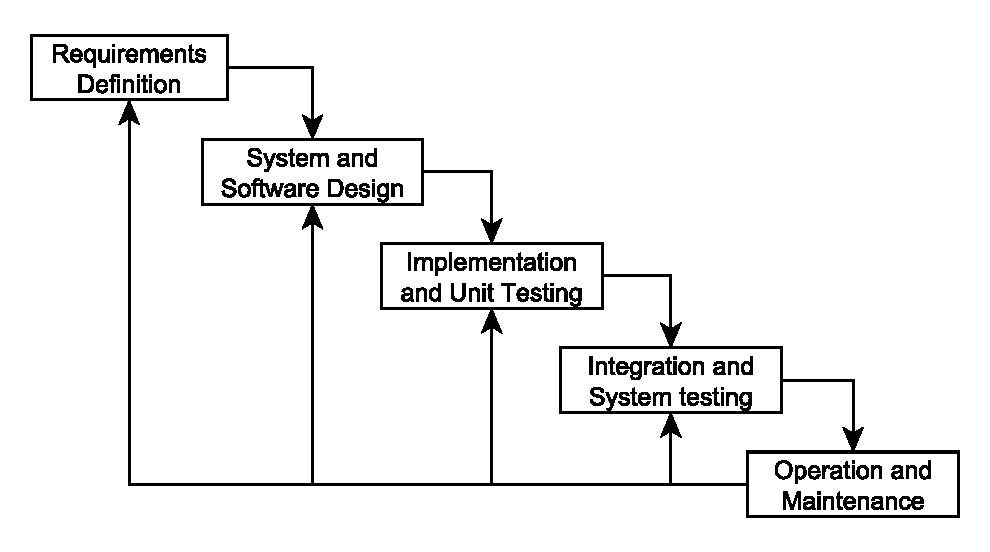
\includegraphics[width=150mm]{images/chapters/development_models/waterfall.pdf}
\caption{The Waterfall model.}
\label{waterfall}
\end{figure}

For larger projects, the following steps are suggested:
\begin{enumerate}
	\item System and Software Requirements: The customer is involved with the specification of the scope and requirements of the system. The resulting documentation serves as a foundation to the next stages of development.
	\item Analysis and Program Design: The requirements produced in the previous stage are used to create a system plan and various design documents.
	\item Coding and Testing: The actual implementation of the project. This also involves continuously testing on various levels (for example unit and integration).
	\item Operation and Maintenance: Once the project has been completed, it has to be maintained during its usage. In addition to improving the program in various ways, this may also involve the inclusion of extra features if the customer so desires. These features can in themselves use the Waterfall model.
\end{enumerate}

The model initially suggested by W. W. Royce discusses a linear model in which each of the aforementioned stages are used as distinct steps in the development process. Each stage is required to be completed before the next is started. This may be a sound premise in theory, but as suggested in the paper it is likely to fail in practice. The argument used is that often during development, unforeseen problems in the design are encountered. The linear model does not allow for a return to a previous stage in development. Hence, it does not allow for changes in the design that could potentially resolve such problems.

Therefore, an alternative model is suggested that allows for the process to return to earlier stages if necessary. This may not be an ideal solution either, but it does allow for encountered problems to be addressed during development.

\subsection{Agile Software Development}

As can be seen from the ending of the Waterfall-section there were doubts about its applicability already at an early stage. With the advancement of business needs and customer involvement something had to change. This opened the door for the introduction of a new software development methodology, namely agile software development. This new way of thinking tries to deal with collaboration in a way that promotes adaptive planning, early delivery and continuous improvement, making the development phase faster and more flexible regarding changes \cite{abrahamsson2002}.

\subsubsection{Scrum}

In this section an introduction to one of the most popular agile software development methodologies will be carried out based mainly on Abrahamsson, Salo, Ronkainen and Warsta's publication on agile methods \cite{abrahamsson2002}, the so-called Scrum. In VersionOne's ``7th Annual State of Agile Development Survey'' Scrum or Scrum variants had a quoted 72% usage making it by far the most popular agile methodology in the survey \cite{Com2013}.

Scrum is an iterative and incremental software development model (as shown in figure \ref{scrum}). It has come forth from the realisation that development methods that were common at the time of its introduction worked well in theory but did not in practice. These methods, Waterfall included, were designed to provide a structured and well-defined development process \cite{scrum}.

The agile software development processes, like Scrum, are part of a recent approach to software development. The idea with Scrum in particular is to divide the development into short periods called ``sprints''. This is done to focus effort for a limited time on short-term goals. Iterating over these goals allows the process to adapt the development plan based on progress but also to address any design problems that arise.

In short, the team concentrates on isolated parts, and through this prioritises on the most important tasks of the project first. The time span of a sprint is typically between one and four weeks long.

In order to implement the requirements step by step and in an orderly fashion, a repository is kept containing the features that have yet to be implemented. This repository is called the ``product backlog''. During development, the requirements could change over time. Therefore the product backlog is not static; it changes to the needs of the project with new topics being added, and obsolete ones being removed. The items from the backlog that a team works on during a sprint is called the ``sprint backlog''.

Meetings are also a key part of Scrum. There are several different types of meetings: sprint planning meeting, daily scrum meeting, backlog refinement, end of cycle and Scrum-of-Scrums. The sprint planning meeting is held at the beginning of each sprint cycle. Here the focus is on what work is to be done, and the sprint backlog for the coming sprint cycle is set. The daily scrum meeting, also called the daily stand-up, is a daily encounter (15 minutes) where each member of the project team answer these three questions:

\begin{enumerate}
  \item What have you done since yesterday?
  \item What are you planning to do today?
  \item Are there any impediments in your way?
\end{enumerate}

Further, there is the backlog refinement, also called ``grooming''. This is where tasks are created, large tasks are decomposed into smaller ones, tasks are prioritised, and the existing tasks are sized in the product backlog. Backlog refinement is often split into two meetings. In the first meeting the product owner and other stakeholders create and refine stories in the backlog. In the second meeting the project team sizes the tasks in the backlog to make them ready for the next sprint. Planning poker is an example of how this can be carried out.

The last listed meeting occurs at the end of each cycle, and is therefore called end of cycle (meeting). This is actually two meetings: a sprint review meeting and a sprint retrospective. At the sprint review meeting the work that is completed and yet to be finished is reviewed. The completed work is also presented for the stakeholders, often called  ``the demo''. At the sprint retrospective all members reflect on the past sprint. Two main questions are answered:

\begin{enumerate}
  \item What went well during the sprint?
  \item What could be improved in the next sprint?
\end{enumerate}

The Scrum team usually consists of five to nine members. It is important to note that Scrum teams do not use traditional roles such as programmer, tester, designer or architect. Instead the main goal for the Scrum team is to collectively complete the tasks within the sprint.

\begin{figure}[ht!]
\centering
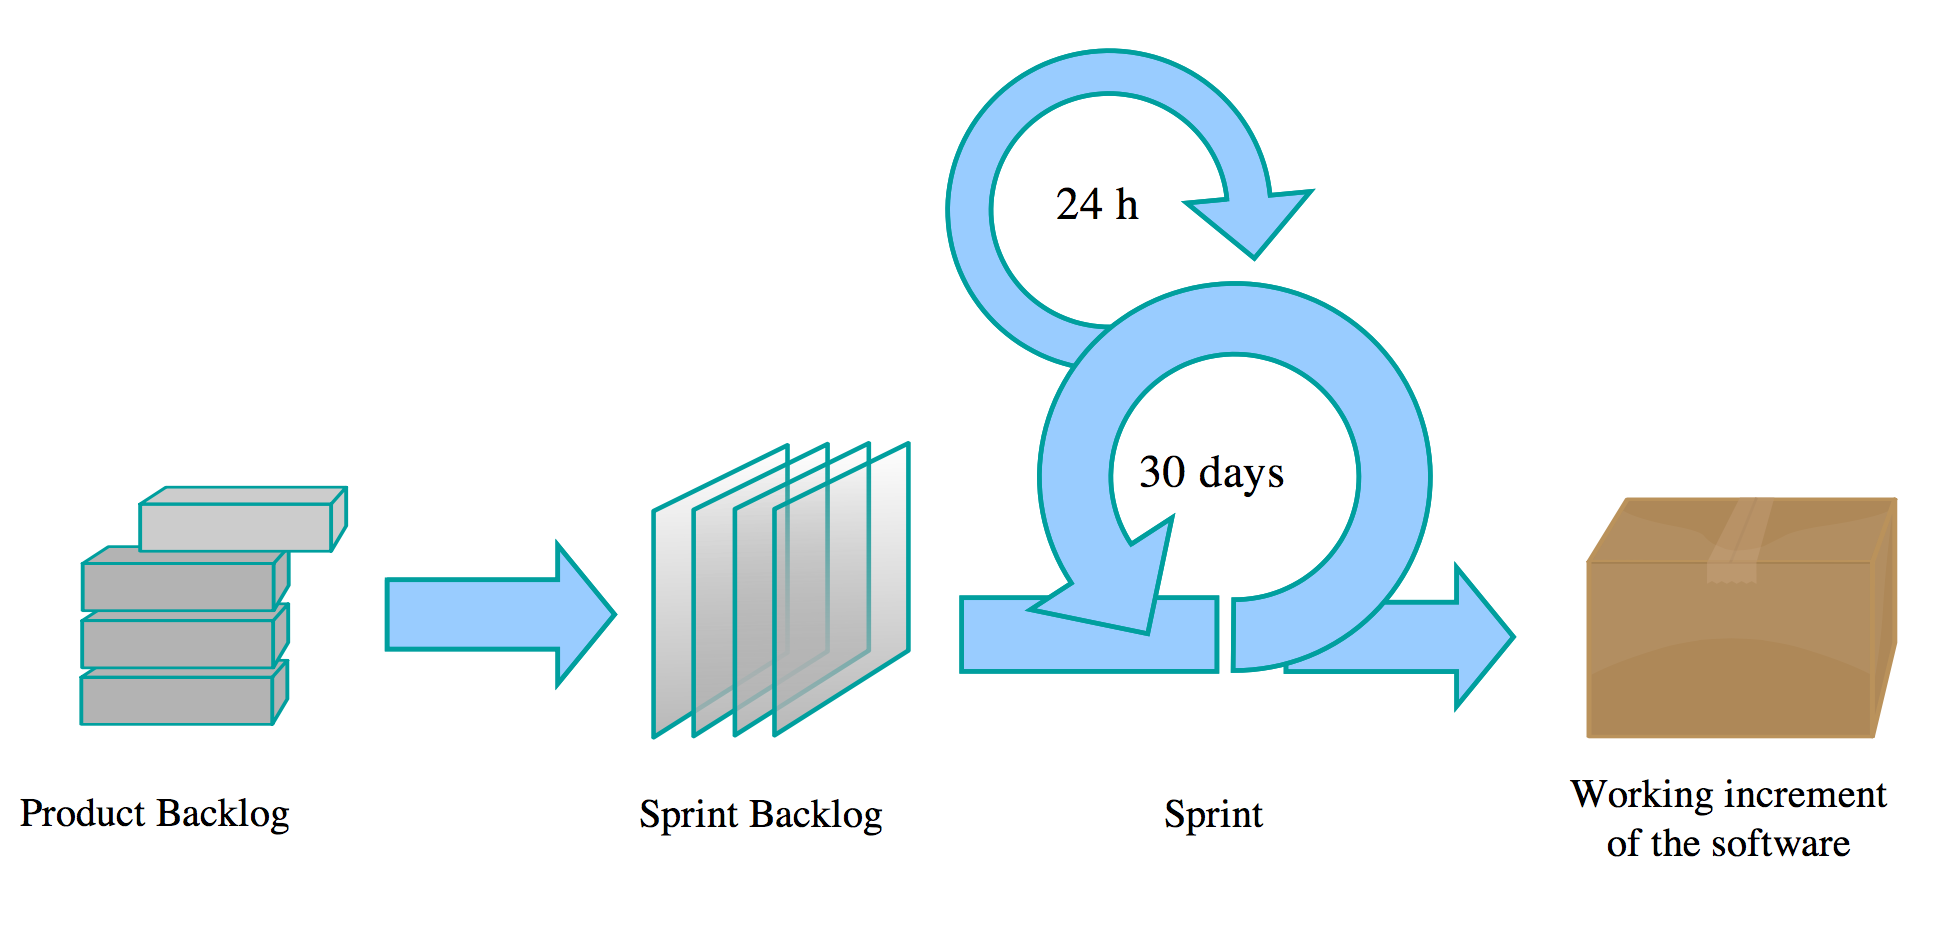
\includegraphics[width=150mm]{images/chapters/development_models/Scrum.png}
\caption{The Scrum cycle.}
\label{scrum}
\end{figure}

To end the section, as well as making a natural shift towards the next topic (Coordination), a look at Scrum-of-Scrums is carried out.

%\subsubsection{

\section{Coordination}



\section{Large-scale}

What is actually ``large-scale''? This was a topic brought up at a workshop regarding research challenges in large-scale agile software development where opinions ranged by some margin. Some suggestions were project duration, project cost, people involved, number of remote sites and number of teams \cite{Dingsoyr2013b}. This issue was further analysed by Dingsøyr, Fægri and Itkonen trying to work out a taxonomy of scale for agile software development. Their results are summarised in table \ref{Scale} where the taxonomy of scale is based on the amount of teams involved in the development project \cite{Dingsoyr2013a}.

\begin{table}[H]
\begin{center}
    \begin{tabular}{| l | l | p{7cm} |}
    \hline
    Level & Number of teams & Coordination approaches \\ \hline
    Small-scale & 1 & Coordinating the team can be done using agile practices such as daily meetings, common planning, review and retrospective meetings. \\ \hline
    Large-scale & 2-9 & Coordination of teams can be achieved in a new forum such as a Scrum of Scrums forum. \\ \hline
    Very large-scale & 10+ & Several forums are needed for coordination, such as multiple Scrum of Scrums. \\
    \hline
    \end{tabular}
    \caption{A taxonomy of scale of agile software development projects.}
    \label{Scale}
\end{center}
\end{table}

Others have also discussed the problems regarding large-scale. For example Schnitter and Mackert discuss the scaling of Scrum at SAP AG and concludes that in their case the maximum involved development employees that may be organised with regards to agile project management is 130 (This number sums up developers in 7 teams (max. 70 people), the product team (max. 16), development infrastructure responsibles (about 10), quality assurance and testers (about 25), general management (about 10)) \cite{Nord2011}.

Another example is taken from Nord et al. defining large-scale by scope of the system, team size, and project duration. They say that the size of the development team must be more than 18 people and distributed into a few teams \cite{Robert2014}.

So the definition of a ``large-scale agile project'' used in this research will be:

\begin{fancyquotes}
An agile project must consist of a minimum amount of two teams coordinating across the teams to be categorised as large-scale.
\end{fancyquotes}

\section{Productivity and Efficiency}